\chapter{Foundation}
\label{cha:foundation}
This chapter will cover the basic knowledge about fingerprinting. First the term fingerprint will be explained and what it can be used for. Further, the threat it poses as well as suggestions on how to reduce a fingerprint will be discussed before covering technologies which can be utilized to track the user. After the base has been layed the chapter closes with the description of the different fingerprinting methods and techniques.

\section{Fingerprinting}
\textit{Web browser fingerprinting}, also known as device fingerprinting, is the systematic collection of information to identify and later re-identify users. (\textcite{doty18}, p.3)(\textcite{amiunique})\\
This data tracking method works by obtaining data from the user's web browser and using this data to create an unique fingerprint "hash". This hash is the key for later re-identifying the user. (\textcite{upi15}, p. 1)(\textcite{havens16}, p. 4)\\\\
With millions of computers and mobile devices in use and even more browsers, this identification method seems really unlikely to work at first sight. Nevertheless, it is an extremely reliable method for correlating data across websites or even web browsers with individual users. (\textcite{havens16}, p. 3)\\
\begin{tcolorbox}
	Example on how it works:\\
	There are currently over 7.5 billion people populating our planet. Imagine you have to identify a single person. By stating this specific person is male, you already cut the choice in half. Information about the ethnicity and age of this person, as well as the time zone he lives in will narrow down the choice even more.\\
	It's basically the same with web browser fingerprinting. The gender can be seen as an equivalent of the used operating system, the ethnicity as the browser and age as the browser version. Information about the time zone and used language are easily acquired by the browser and so are more specific details which help narrowing down the choice to one person.
\end{tcolorbox}

This combination of properties can be obtained using code (time zone, screen resolution, plug-ins) and also be extracted from HTTP headers (user agent string). (\textcite{miele18}) \\\\
Web browser fingerprinting was first developed short before 2010 and due to its effectiveness quickly gained traction in the tracking industry. (\textcite{havens16}, p. 3) \\
Many of the fingerprinting methods can not be detected by the user, and as it is extremely difficult for users to modify their web browsers in a way that they are less vulnerable to it (\textcite{amiunique})(\textcite{miele18}), makes it a dangerous tool for deanonymization attacks and maliciously-minded tracking programs. (\textcite{havens16}, p.3)\\
\begin{tcolorbox}
Example:\\
Upon accessing a website, the fingerprinting script determines the user's fingerprint and pushes it to a central data store. This data store is usually a shared data store which is used by multiple websites. So when the user accesses another website, which also has access to this specific shared data store, the user will be recognized and the user profile can be updated. (\textcite{havens16}, p. 8)
\end{tcolorbox}

\begin{comment}
Web browser fingerprinting is a tracking method, which can correlate user's browsing activity within as well as across sessions without transparency or control. (\textcite{doty18}, p---) Most fingerprinting techniques are obscure and users usually don't notice that they are being tracked.\\\\
The modern web exposes a number of details about the user’s device, either directly or discoverable through testing. This is largely a result of a greater need to comply with different device types, support for different features, or simply leaking data by including too much information in protocol requests. (\textcite{havens16}, p. 4)
\end{comment}
%\subsection{Entropy} - (\textcite{khan14})
\section{Utilisation}\label{sec:utilisation}
In a study conducted in 2013 by Nikiforakis et al. they found that fingerprinting is a part of some of the most popular websites on the internet and that multiple hundred thousands of users are fingerprinted on a daily basis. (\textcite{nikiforakis13}, p.6) \\\\
The following paragraphs lists different ways in which fingerprinting can be utilized:\\\\
Constructive use
\begin{itemize}
	\item Security authentication\\
	Using web browser fingerprinting to correctly identify a device which is used to log into an account can be used to re-identify a user and help combat fraud or credential hijacking. (\textcite{upi15}, p.4)(\textcite{nikiforakis13}, p.2)
	\begin{tcolorbox}
	Example:\\
	Services can track the devices used to access an account and inform the user in case an unknown device tries to access it. 
	\end{tcolorbox}
\end{itemize}
Destructive use
\begin{itemize}
	\item Hacking\\
	Habits of users can be tracked without their knowledge and attackers can acquire specific knowledge about the user’s software setup. (\textcite{upi15}, p.4) 
	\begin{tcolorbox}
	Example:\\
	With the help of web browser fingerprinting a hacker can acquire knowledge about the users operating system and adjust his hacking method accordingly.
	\end{tcolorbox}
\end{itemize}
Con- and destructive use
\begin{itemize}
	\item Identifying criminals\\
	As a mean of tracking, fingerprinting can be used to track people or even criminals. But as seen in the previous examples this can be used to harm or benefit users. 
	\begin{tcolorbox}
	Example: positive use\\
	When a user A is harassed or stalked by another user B, the website can use web browser fingerprinting as a mean of blacklisting said user B. 
	\end{tcolorbox}
	\begin{tcolorbox}
	Example: negative use\\
	Citizens of countries with a strict regime can be blacklisted for expressing criticism against the government.
	\end{tcolorbox}
	\item Commercial use\\
	Commercial fingerprinting is used to track people’s habits and preferences. The acquired knowledge can be used to either help the user or direct him into a certain direction. 
	\begin{tcolorbox}
	Example: positive use\\
	A website picks up the user’s habit to look for climbing gear and suggests similar products.
	\end{tcolorbox}
	\begin{tcolorbox}
	Example: negative use\\
	A website registers that the user recently bought more expensive products and starts to only show items in this certain price range rather than more suitable but cheaper products.
	\end{tcolorbox}
\end{itemize}
The following paragraphs will summarize the findings of a study conducted by Nikiforakis et al. in cooperation with three commercial fingerprinting companies in order to test multiple websites for the use of fingerprinting scripts.\\\\
Nikiforakis et al. used the categorization of TrendMicro and McAfee on a list of 3804 domains. If a domain was neither analysed nor categorized by both used services they were marked as untested and not used. Therefore only 59.2\% of the 3804 domains were included in the results of this testing. If one service declared a domain as unsafe and the other stated the opposite, it was accepted as safe. Some categories were given aliases and gathered in a more generalized category.(\textcite{nikiforakis13}, pp.6)\\
\begin{figure}[H]
\centering
		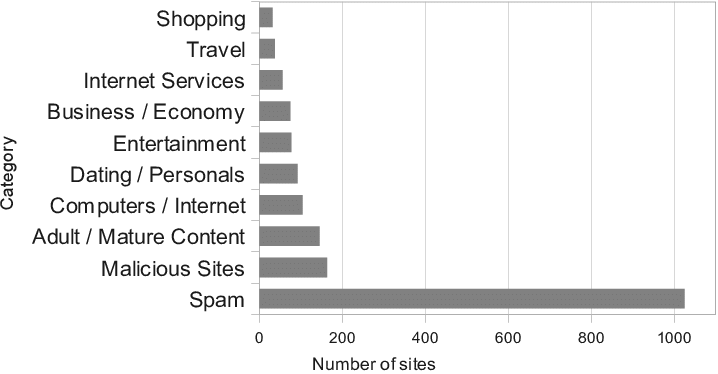
\includegraphics[width=350pt, height=160pt]{Top10CategoriesNiki.png}
		\caption{Top 10 categories utilizing fingerprinting (\textcite{Top10Niki})}
		\label{Top10Niki}
\end{figure}
\autoref{Top10Niki} shows 10 categories, 8 of which operate with user subscriptions. These sites usually are interested in preventing hijacking of user accounts and fraudulent activities.\\
The top two categories were identified as malicious (163 domains) or as spam (1063 domains). Nikiforakis et al. noticed that many domains belonging to one of these categories were parked websites which do not include any fingerprinting code. Further, many "quiz" or "survey" websites were discovered which extract a user's personal details. The domains were categorized as malicious if they exploit vulnerable browsers or extract private data from users. (\textcite{nikiforakis13}, p.7)\\\\
It was discovered that all these sites were found to include, at some point, fingerprinting code provided by one of the three commercial fingerprinting companies.\\
This observation, paired with the fact that all three studied providers stated that there must be made an appointment in order to acquire fingerprinting services, point to the possibility that fingerprinting companies work with dubious domains in order to expand their fingerprinting database. (\textcite{nikiforakis13}, p.7)

\section{Threat}
As seen in the previous \autoref{sec:utilisation} web browser fingerprinting can be utilized in destructive ways. This section will take a closer look at the threat fingerprinting poses for the user's privacy and security.\\\\
The most tricky part about fingerprinting is, that on the one hand users usually do not know that they are being tracked, and on the other hand they can't do anything to prevent it (see \autoref{mitigation}). (\textcite{upi15}, p.4) \\\\
So for example P. Eckersley was able to generate unique fingerprints for 83.6\% of 470,161 browsers that belong to users who have a high awareness of privacy concerns. (\textcite{eckersley10}, p.2,8)\\\\
Even though the fingerprint can change due to modified characteristics, there is a simple algorithm to detect these changes. With heuristics this algorithm was able to re-identify a changed fingerprint with 99.1\% accurancy out of 65.56\% guesses of changed fingerprints.(\textcite{eckersley10}, p.13)\\\\
Below are a few threats listed which fingerprinted users might face:
\begin{itemize}
	\item due to the possibility of being identified some users might face surveillance, risk their personal physical safety or concerns about discrimination due to their internet activities. (\textcite{doty18}, p.4)
	\item the tracking enables collection without clear indications that such a collection is happening without clear or effective user controls. (\textcite{doty18}, pp.4)
	\item Tor enables JavaScript by default and if the user fails to turn it off, even Tor users can be tracked due to the information leaked by JavaScript. (\textcite{havens16}, pp.9)
\end{itemize}

\subsection{Under General Data Protection Regulation}
This threat posed by web browser fingerprinting as depicted above might be reduced by the \textit{General Data Protection Regulation (GDPR)}, which entered into force on May 25th 2018. This regulation imposed by the European Union (EU) intends to cover this kind of hidden data collection, which is used by web browser fingerprinting by forcing companies to prove they have a legitimate reason for the utilization of any means of tracking. (\textcite{miele18})\\\\
Even though the GDPR avoids specifying technologies, it provides general rules which should keep up with technological development. Due to this regulation browser characteristics are now to be treated like personal data. Personal data has a broad definition, as any information that might be linked to an identifiable individual can be passed as such. Examples for such are not only the IP-Address and MAC-Address of users but also less specific features, including the combination of characteristics which web browser fingerprinting relies upon. (\textcite{miele18})\\\\
In order to be allowed to use fingerprinting legally the concerned entity has to complete the following steps:
\begin{itemize}
	\item show that the tracking does not violate the fundamental rights and freedoms of the data subject, including privacy, 
	\item and is in line with reasonable expectations of data subjects
	\item further, give a legitimate argument for its interest in tracking,
	\item and share details about the scope, purposes, and legal basis of the data processing with the person subjected to the fingerprinting.
\end{itemize}
Due to this regulation, the only step the user has to take to avoid fingerprinting is to say "no".\\\\
Even though the rules imposed by this regulation seem to help prevent unwanted tracking, it only helps mitigate it. There will certainly be fewer entities making use of fingerprinting, though web browser fingerprinting is not expected to disappear, no matter how high the penalties are on its illegal utilisation.\\\\
Anyway, the GDPR only applies on processed personal data of individuals living in the \textit{European Economic Area (EEA)} for commercial purposes, or for any purposes when the behaviour is within the EEA. There will always be companies which either think they can escape the consequences or which claim to have "legitimate interest" in tracking users. Furthermore, no matter how strict regulations are, it always comes down to the user. Due to the plentiful requests for consent as they are found on the web nowadays many users are worn out and do not take a second look at the privacy policy regulated by the GDPR. (\textcite{miele18})

\section{Mitigation} \label{mitigation}
As seen in the previous sections there are many ways of utilizing web browser fingerprinting. Many of these possible applications pose a threat to the user's privacy which brings up the question if it can be avoided. Each of the researched papers about this topic states the same - No. Unfortunately, it is impossible to opt-out fingerprinting. (\textcite{web17})(\textcite{upi15}, p.4)\\\\
Even if it is not possible to prevent the possibility of being fingerprinted, there are many suggestions on how to at least mitigate the characteristics which are used to generate an unique fingerprint. Some of these suggestions are stated below:
\begin{itemize}
	\item Blocking tools which are maintained by regular web-crawls to detect tracking and incorporate blocking mechanisms (\textcite{acar14}, pp.11);\\
	\textit{This might work with active fingerprinting methods but not with the passive methods.}

	\item Having Flash provide less system information and report only a standard set of fonts (\textcite{nikiforakis13}, p.13);\\
	\textit{This would require Flash developers to take enough interest in this topic to change security settings. It might also cause rendering problems.} 
	%%???
	
	\item Use private browsing modes or Tor anonymity service;\\
	\textit{Tor is slower and while it disables WebGL it still allows rendering to the <canvas> element which partly exposes the user to canvas fingerprinting.} (\textcite{mowery12}, p.1)
	
	\item Browser vendors agree on a single set of API calls to expose to the web applications as well as internal implementation specifics (\textcite{nikiforakis13}, p.13);\\
	\textit{This would require all browser vendors to take enough interest in this topic to change their API calls.}
	
	\item Browser vendors agree on an universal list of "canvas-safe" fonts (\textcite{mowery12}, p.10)(\textcite{boda11}, p.16);\\
	\textit{This would again require the cooperation of all browser vendors. If only a few browsers adapt their settings this might make them more distinct.} 
	
	\item Support WebGL which ignore graphic cards and render scenes in a generic software renderer;\\
	\textit{This approach might be good while the performance impact is not.} (\textcite{mowery12}, p.10)
	
	\item Require the users approval whenever a script requests pixel data (\textcite{mowery12}, p.10);\\
	\textit{The reason why the approval is needed might be covered. Further, a casual user will not know the effects of accepting.}
	
	\item Modification of the user agent string;\\
	\textit{Opinions vary on this ones. While Yen et al. claim that this measure helps, Nikiforakis et al. as well as other authors state otherwise.} (\textcite{yen09}, p.5) (\textcite{nikiforakis13}, p.13) (\textcite{eckersley10}, p.4)
	
	\item Decrease the verbosity of plug-in versions and the user agent string (\textcite{boda11}, p.16);\\
	\textit{This measurement might help to reduce the uniqueness of said characteristics.}
	
	\item Enable the user to set fake system properties in browser like hiding the operating system, time zone and screen resolution (\textcite{boda11}, p.16);\\
	\textit{This measurement might increase the fingerprintability if the real properties leak or are maliciously set.}
	
	\item Browser extension which automatically blocks active content e.g. NoScript, ScriptBlock (\textcite{web17}) \\
	\textit{Helps against canvas fingerprinting but does not prevent passive methods.}
	
	\item Use commonly-used web browsers and default settings, including the operating system (\textcite{web17});\\
	\textit{Good suggestions as no fingerprinting technique is able to distinguish identically configured devices.}	
\end{itemize}

\begin{comment}
N. Doty suggested a few best practices in his paper "Mitigating Browser Fingerprinting in Web Specifications" such as the following (\textcite{doty18}, pp.10):
\begin{itemize}
\item Avoid unnecessary or severe increases to fingerprinting surface
\item Mark features that contribute to fingerprintability
\item Specify orderings and non-functional differences
\item Design APIs to access only the entropy necessary
\item Enable graceful degradation for privacy-conscious users or implementers
\item Avoid unnecessary new local state mechanisms
\item Highlight any local state mechanisms to enable simultaneous clearing
\item Limit permanent or persistent state\\
\end{itemize}
Further Doty mentions that this helps (\textcite{doty18}, p.6): 
\begin{itemize}
\item Decreasing fingerprinting surface
\item Increasing anonymity set
\item detectable fingerprinting
\item clearable local state
\end{itemize}
While N. Doty only listed ways to decrease the chance of being fingerprinted, R. Upathilake suggests the following steps to actually prevent the chance of being tracked via web browser fingerprinting (\textcite{upi15}, p.4):
\end{comment}
\section{Critical Technologies} \label{sec:technologies}
\begin{comment}
%https://www.1and1.ca/digitalguide/online-marketing/web-analytics/browser-fingerprints-tracking-without-cookies/
\begin{figure}
	\centering
	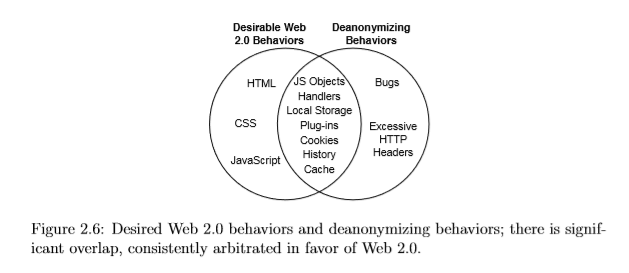
\includegraphics[width=0.7\linewidth]{images/dangerousConfigs}
	\caption{}
	\label{fig:dangerousconfigs}
\end{figure}
(\textcite{mayer09}, p.43)
\end{comment}
As mentioned in the previous sections scripts which use fingerprinting can read certain data via configuration settings or other observable characteristics from the web browser, which enables them to create a specific fingerprint. (\textcite{doty18}, p.3) The following paragraphs will outline some of these configurations. 

\begin{comment}
The information that browser fingerprinting reveals typically includes a mixture of HTTP headers (which are delivered as a normal part of every web request) and properties that can be learned about the browser using JavaScript code: your time zone, system fonts, screen resolution, which plug-ins you have installed, and what platform your browser is running on. Sites can even use techniques such as canvas or WebGL fingerprinting to gain insight into your hardware configuration.(\textcite{miele18})
\end{comment}
\subsection{JavaScript}\label{JS}
JavaScript is a web development language for web functionality. (\textcite{wood}) It allows client-side scripting and gives access to many browser-populated features like the installed plug-ins. (\textcite{amiunique}) It is enabled by default in all major browsers and by November 2018 JavaScript was included by 95\% of all websites online. (\textcite{jsinfo}) (\textcite{w3techs18})\\\\
JavaScript can be executed on any device which has a \textit{JavaScript Engine}. (\textcite{mulazzani13}, p.2) (\textcite{jsinfo}) This engine is responsible for parsing the script to compile it into machine language which can be exeucted. During this process the engine applies optimizations on every state of the process. (\textcite{jsinfo})\\\\
Known JavaScript Engines:
\begin{itemize}
	\item V8 in Chrome and Opera
	\item SpiderMonkey in Firefox
	\item ChakraCore for Microsoft Edge\\\\
\end{itemize}
JavaScript Engines usually implement features which are specified by \textit{ECMAScript} .  (\textcite{jsinfo})(\textcite{mulazzani13}, p.2)\\
ECMAScript provides rules, details, and guidlines which have to be regarded for a scripting language in order to be ECMAScript compliant. It is represented by ECMA-262, which is a standard published by Ecma International (responsible for creating standards for technologies). (\textcite{aranda17})\\\\
In-Browser JavaScript is seen as "safe" programming language as it only has a low-level access to memory or CPU. Its abilities are therefore limited and it has no direct access to OS system functions. (\textcite{jsinfo})\\\\
Nevertheless, can JavaScript also be used to retrieve browser characteristics like the user's time zone and system color. Further there are two properties which can be used to acquire additional information about the user's screen and window.(\textcite{web17})\\\\
The \textit{navigator object} is a possible property for window objects and supported by all major browsers. Informations which can be acquired through the navigator object include: browser name and version, if cookies are enabled, browser language, platform and the useragent (which does not differ from the user agent in \autoref{UAS})(\textcite{web17})\\\\
The \textit{screen} is a property which holds information about the user's screen. For example the screen width and height, the acutal available display width and height and the color depth which is supported by the user's device.(\textcite{web17})\\\\
When JavaScript is disabled, websites are not able to detect the list of active plug-ins and fonts, and neither will be able to install certain cookies on the targeted browser. The disadvantage of disabling JavaScript is that websites won’t always function properly, because it is also used to make websites run smoothly and therefore will impact the browsing experience.(\textcite{pixel18})

%has some tests which e.g. are later used for js engine fp -- what is sputnik and test 262 ()
%one of the fastest evolving languages, in terms of practices, tooling, n ecosystem (\textcite{wood})

\subsection{Adobe Flash}\label{adobe}
Adobe Flash is a proprietary browser plug-in which provides different ways of delivering rich media content which is usually not displayed in HTML. (\textcite{nikiforakis13}, pp.2) It used to be the most commonly used video format on the internet but can now be replaced with safer technologies like HTML5 (see \autoref{html5}). Even though it could be replaced, it is still installed on the vast majority of browsers. (\textcite{web17})(\textcite{nikiforakis13}, p.3) \\\\
This plug-in can be used to retrieve sensitive data from the user, for example can it detect HTTP proxies. Besides, has it reimplemented certain APIs which already exist in browers and are accessible through the use of JavaScript (see \autoref{JS}). (\textcite{nikiforakis13}, p.2) This rich programming interface (API) can be used to access system-specific attributes, such as the operating system and its version, a list of fonts, screen resolution and time zone.(\textcite{amiunique})(\textcite{havens16}, p.5) Furthermore, the API does not provide the same result as the original browser API, but even more detailed return values. (\textcite{nikiforakis13}, p.2)
\begin{tcolorbox}
	Example: \\
	Firefox might return “Linux x86 64” if it is queried about the platform execution while Flash might provide the full kernel version "Linux 3.2.0-26-generic". (\textcite{nikiforakis13}, p.2)\\
\end{tcolorbox}
Apart from these security risks is Adobe Flash also being criticized for its poor performance, as well as lack of stability. (\textcite{nikiforakis13}, p.3) Another vulnerability is its local storage objects which enable so called \textit{zombie cookies}. These zombie cookies populate in various storage locations on the targeted device and re-populate in case one of these storage areas is cleared. These cookies can also be used paired with fingerprinting in order to keep track of changes in fingerprints ("cookie syncing"). (\textcite{havens16}, p.8f)\\\\
Adobe Flash can be disabled or even uninstalled which might effect the user experience on old websites negatively. (\textcite{pixel18})

\subsection{HTML 5}\label{html5}
HTML5 is the latest version of the Hypertext Markup Language, which is a coding language used to build websites and supported by all major browsers. (\textcite{pixel18})(\textcite{marshall17}) It can be used to build complicated applications, as well as provide animations, movies, music, and the likes. This without the need of any additional software (plug-ins). Summed up, it provides features like geolocation, graphics, video and webapps. (\textcite{marshall17})\\\\
Apart from its incredible capabilities there is a slight problem concerning HTML5 video. As it would not be agreed upon which format(s) should be supported, which ended in each browser supporting different HTML5 video formats.\\
As HTML5 does not include digital rights management technology which is used to prevent the user from copying the content, content owner usually prefer Adobe Flash (see \autoref{adobe}). (\textcite{marshall17})\\\\
One of HTML5's new elements is <canvas> element which is used to draw graphics on a web page.(\textcite{pixel18}) Through this process, it is possible to acquire any differences in the hardware and software configurations due to slight image rendering differences. (\textcite{amiunique}) This provides a way to inspect the data with pixel accuracy which later can be used in fingerprinting techniques like described in \autoref{canvasfp} (\textcite{mowery12}, p.2) \\\\
In \autoref{canvasfp} \textit{Base64 encoded images} are used which is one of the oldest ways to encode something in html. Base64 encoded images are a part of the HTML and enable the website to display the images without loading. It turns different types of data into a combination of numbers and letters which is safe for HTML. One of the main benefits is that the webpage does not have to load an external ressource which helps the page to load faster. This performance benefit only works if small images are used. (\textcite{sexton15})

\subsection{User agent}\label{UAS}
A user agent is a request header field in the hypertext transfer protocol (HTTP) which is used for the communication between browser and website. (\textcite{xovi18}) It is automatically sent with each page call, except if specifically configured not to. (\textcite{xovi18})(\textcite{fielding14}, p.5.5.3)\\\\
The user agent contains the name and version of the used browser. In R. Fielding's work about HTTP, this combination is also called \textit{product identifier}. The product identifiers are listed in the order of their importance, whereas each of them can be followed by one or multiple comments. (\textcite{xovi18})(\textcite{fielding14}, p.5.5.3) This field value is often called user agent string. (\textcite{hoffman16})\\
\begin{tcolorbox}
Example 1: \\
Mozilla/5.0 (Windows NT 10.0; WOW64) AppleWebKit/537.36 (KHTML, like Gecko) Chrome/69.0.3497.102 Safari/537.36 Vivaldi/2.0.1309.37
\end{tcolorbox}
This string tells the receiving server, that the latest version (2.0.1309.37) of the Vivalid browser is used. In the comments (contained in the brackets) it gives away that the computer runs Windows 10 (Windows NT 10.0) on a 64-bit version (WOW64).\\
\begin{tcolorbox}
Example 2:\\
Mozilla/5.0 (Windows NT 10.0; Win64; x64) AppleWebKit/537.36 (KHTML, like Gecko) Chrome/64.0.3282.140 Safari/537.36 Edge/17.17134\\
\end{tcolorbox}
Similar to the first example, this browser (Edge with the version number 17.17134) also gives away the operating system and its version (same as before).\\\\
As shown in the examples above, not only the used browser name and its version are passed on, but also information about the operating system and sometimes hardware. (\textcite{hoffman16}) (\textcite{xovi18}) The passed-on information is used to display different content in different browsers, on different operating systems or to gather statics (\textcite{hoffman16}) (\textcite{arntz17}) (\textcite{xovi18})\\\\
If wanted, changes on the user agent string can easily be made. (\textcite{arntz17})
The problem with this configuration is, that the longer the user-agent field values become, the higher becomes the risk of being identified through for example fingerprinting. Therefore, the user should limit the addition to the user-agent string which can be requested by third parties. (\textcite{fielding14}, p.5.5.3)

\begin{comment}
\subsection{Others}
In the previous 
Quickly describe which else there are:
(\textcite{havens16}, p.5):
Language – Language the browser is in; used for localization
Screen Resolution – the with and height of the user’s screen
// here reference to why ratio is better -> zoom
Timezone – the local timezone of the user’s computer
DoNotTrack – weather the user has indicated they wish to opt-out of tracking
Installed Fonts – the fonts supported in the browser, typically retrieved from Adobe Flash but can also be detected by other means
Canvas Fingerprinting – The program attempts to render an image on the webpage using the HTML5 canvas. Subtle differences in the rendering of the image can lead to identification

(\textcite{havens16}, p.6)
Browser plug-ins – a list of plug-ins installed in the browser
Cookies enabled – whether or not the user allows cookies on the page
Benchmark tests – evaluate how the browser’s js engine performs against a list of published bench marks. This information is often used to supplement that of the user agent string

\subsubsection{WebGL}\label{webgl}
%WebGL provides a JavaScript API for rendering 3D graphics in a <canvas> element. Modeled after OpenGL ES 2.0, WebGL is currently a draft specification and implemented and enabled in Chrome, Firefox, and Opera, as well as implemented but disabled in Safari. Each of these browsers provides a hardware-accelerated implementation, using the installed graphics hardware to render each frame. To mitigate serious misbehaviour and crashes, all of these browsers enable WebGL only for a whitelisted set of graphics cards and drivers.
%Current WebGL implementations expose their functionality through a separate canvas context (which will eventually be named “webgl”). The WebGL API is too complex to describe here in sufficient detail, but is stylistically similar to the desktop OpenGL API. It provides for vertex and fragment shaders, written in OpenGL Shading Language (GLSL), that, after compilation, run directly on the graphics card. WebGL also provides for OpenGL-style textures, as well as different lighting primitives. More advanced techniques, such as specular highlighting, bump mapping, and transparency, can be achieved through custom GLSL shaders. 2.4 SecurityImplications 
%(\textcite{mowery12}, p.3)
\end{comment}

\section{Web browser fingerprinting methods}\label{sec:Methods}
\subsection{Active fingerprinting}
Active fingerprinting actively queries information about the client by running JavaScript code or using plug-ins like Adobe Flash which extend the browsers functionality. (\textcite{web17})((\textcite{doty18}, p.6)\\\\
Some of the additional characteristics which can be retrieved with this method are:
\begin{itemize}
	\item user's screen (width, height, resolution)
	\item window size
	\item enumerating fonts
	\item time zone
	\item plug-ins
	\item evaluating performance characteristics
	\item rendering graphical patterns\\
\end{itemize}
The only potential disadvantage active fingerprinting provides, is that it can be detected on the client-side in case the user analyses the outgoing data packages, HTML or the JavaScript source code. However, this does not happen in the majority of cases. (\textcite{doty18}, p.6)(\textcite{web17})\\\\
Active fingerprinting techniques
\begin{itemize}
	\item Canvas fingerprinting
	\item JavaScript Engine fingerprinting
	\item Cross-Browser fingerprinting
	\item Browser specific fingerprinting
\end{itemize}

\subsection{Passive fingerprinting}
In contrast to active fingerprinting methods, passive fingerprinting does not need to execute any code on the client side. This method works based on observable characteristics which are contained in the header data of the IP packet by default. (\textcite{doty18}, p.6)(\textcite{web17}) There is no way for the user to learn if a website is using a passive fingerprinting method and is secretly storing data.\\\\
Some of the provided characteristics are:
\begin{itemize}
	\item cookies
	\item HTTP request headers
	\item IP address and port
	\item character sets (e.g. UTF-8)
	\item languages\\
\end{itemize}
Passive fingerprinting techniques
\begin{itemize}
	\item Browser specific fingerprinting
\end{itemize}

\section{Web browser fingerprinting techniques}\label{sec:Techniques}
As described in \autoref{sec:Methods} there are different methods of fingerprinting. These methods are implemented in different techniques which will be discussed in this chapter.
\subsection{Browser specific fingerprinting} \label{specFP}
%can be both active and passive?
In 2010, P. Eckersley conducted a study on the project "Panopticlick" which checks how trackable users are. The tracking is done with the help of a fingerprint which is generated from previously collected data. (\textcite{upi15}, p.2) This study has shown that 94.2\% of the users which use Flash or JavaScript could be distinguished with the help of browser fingerprinting. (\textcite{eckersley10}, p.2)
\subsubsection{How it works}
Browser specific fingerprinting is a technique which only uses browser-dependent features to collect a number of common and less-common known browser characteristics.\\\\
This kind of fingerprinting is possible even if the browser only reveals its version and configuration information which is usually enough to create a distinct fingerprint. (\textcite{eckersley10}, p.16) Although the retrieved browser information typically includes the installed fonts, plug-ins (including version numbers), user agent, HTTP accept and screen resolution. (\textcite{upi15}, p.2)\\\\
As this kind of fingerprint is just a concatenation of this information it is easily affected by changes, like upgrades, newly installed features or external system changes.
Usually, simple heuristics can be used to adjust the browser specific fingerprint accordingly.(\textcite{eckersley10}, p.4) (\textcite{upi15}, p.2)\\\\
In some cases when the user tries to hide browser features, the opposite happens as the fingerprint is made more distinct. See the example below.\\
\begin{tcolorbox}
	Example: \\
	Even when using a Flash-blocking add-on, the browser still displays Flash in the plug-in list. Due to the add-on the list of system fonts can't be obtained, this creates a distinct fingerprint, although the Flash-blocker was not explicitly detected. (\textcite{eckersley10}, p.4)
\end{tcolorbox}
Like many other web browser fingerprinting techniques, browser specific fingerprinting is not able to distinguish instances of identically configured devices. Further, other than cross-browser fingerprinting, this is a single browser fingerprint technique, which means it can not re-identify a user in another browser as the fingerprint may change across browsers. \textcite{upi15}, p.2)

\subsection{Canvas fingerprinting} \label{canvasfp}
Canvas fingerprinting was first mentioned and implemented by Mowery and Shacham in 2012 as part of their work "Pixel Perfect: Fingerprinting Canvas in HTML5".\\ Any website that runs JavaScript on the user's browser can use the HTML5 <canvas> element and observe its rendering behaviour. There is no need for any special access to system resources. (\textcite{mowery12}, p.1)(\textcite{upi15}, p.2)\\\\
The outcome of their research and tests showed that the canvas fingerprint is consistent but can change depending on hardware and software configuration. Only 2 years after its first use, a study conducted by Acar et al. ascertained that canvas fingerprinting is the most common form of fingerprinting with an approximate occurrence of 5.5\% in the top 100,000 Alexa websites. (\textcite{acar14}, p.5)

\subsubsection{How it works}
Canvas fingerprinting renders text and WebGL scenes onto an area of the screen using the HTML5 <canvas> element programmatically. Each browser renders differently which helps acquiring a distinctive part for the fingerprint. So for example, out of 300 samples the text font Arial was rendered in 50 distinctive ways.(\textcite{mowery12}, p.6)\\\\
After rendering the text or WebGL scene using HTML5<canvas> the pixel data is read to generate a fingerprint. Through this process a 2D graphic context is obtained and a text or image is drawn to the canvas.(\textcite{upi15}, p.2)\\
The obtained canvas object provides a toDataURL() method which gives a data url consisting of a Base64 encoding of a png image which contains the canvas' content. This Base64 encoded pixel data url is used to create a hash.(\textcite{mowery12}, p.3)(\textcite{upi15}, p.2)\\\\
Base64 is an encoding standard which is used when binary data needs to be encoded. Basically it works by splitting the given binary input into groups of 6 bit. Using the 64 alphabet table (see \autoref{Base64Alphabet}) each group is depicted by one of the 63 characters in this alphabet.
(\textcite{josef06})
\begin{figure}[H]
	\centering
	\includegraphics[width=350pt, height=180pt]{base64Encoding.png}
	\caption{Base64 Alphabet (\textcite{Base64Alphabet})}
	\label{Base64Alphabet}
\end{figure}
At least the operating system, browser version, graphics card, installed fonts, sub-pixel hinting and anti-aliasing all play a part in the final fingerprint.(\textcite{upi15}, p.2) \\\\
In their paper K. Mowery and H. Shacham used two types of image comparisons to check if the user's configuration matches a fingerprint: \textit{pixel-level difference} and \textit{difference maps}.(\textcite{mowery12}, pp.4)\\\\
Pixel-level difference works by setting each pixel's color to a specific color. If the pixel's color isn't a transparent pure black it indicates that two pixels don't match and therefore its alpha value is set to 255 to render it completely opaque. (\textcite{mowery12}, pp.4)\\\\
Difference maps work in a similar way, only that this method sets a pixel either black or white, depending on whether they differ. If an image is purely white it indicates that they are identical images. (\textcite{mowery12}, pp.4)\\\\
Canvas fingerprinting can not distinguish identically configured devices and can not fingerprint a user across different browsers.(\textcite{mowery12}, p.5) \textcite{upi15}, p.2)

\begin{comment}
%It is transparent to the user. Our tests can be performed, offscreen, in a fraction of a second. There is no indication, visual or otherwise, that the user’s system is being fingerprinted.

Overall, our fingerprints do combine beneficially: 
among the 116 groups, our five extremely simple tests show a distribution entropy of 5.73 bits. We believe that more specialized and targeted tests could reveal even more, perhaps down to the exact installed graphics card, operating system, and browser family. (\textcite{mowery12}, p.8)

It is high-entropy. In 294 experiments on Amazon’s Mechanical Turk, we observed 116 unique fingerprint values, for a sample entropy of 5.73 bits. This is so even though the user population in our experiments exhibits little variation in browser and OS. (\textcite{mowery12}, p.1)

When writing their thesis Mowery et al. did not have access to various hundreds distrinct customer-level computer systems and therefore went to use Amazon Mechanical Turk and were able to collect samples from 300 distrinct member of this marketplace.(\textcite{mowery12}, pp.4) Running 5 fingerprinting tests in the background they collected metadata (browser's user agent string, WebGL-reported renderer, vendor, and version.
\end{comment}
\subsection{JavaScript Engine fingerprinting}
In 2011 P. Reschl et al. published their first paper about the use of the JavaScript Engine to uniquely identify a web browser and its version. Comparing it to the Panopticlick project (\textcite{eckersley10}) it was stated in the paper that the new approach is multiple times faster and less error prone. (\textcite{reschl11}, p.2) Two years later, in 2013, the same team with some additional authors published another paper in which this fingerprint technique was described in more detail.(\textcite{mulazzani13}, p.1) \\\\
Compared to other methods this technique does not rely on the user agent string (which can be modified, see \autoref{UAS}) which makes it a more robust fingerprinting technique.(\textcite{mulazzani13}, p.1)

\subsubsection{How it works}
JavaScript Engine fingerprinting works by running test cases of conformance tests like Sputnik and test262 to identify browsers and their major versions. Even though these test suits consist of multiple thousands test cases the browser only needs to fail one particular test which every other browser passed to be identified. Therefore these fingerprinting technique only needs a fraction of a second to be executed. (\textcite{mulazzani13}, p.3) \\\\
There are two methods which can be used for identification:\\\\
For a rather small test set the \textit{minimal fingerprint method} can be used. First test262 is started for each browser in the set and the results are compared. For each browser a test is selected which only this specific browser failed (uniqueness = 1). This browser can be uniquely identified by this test and is therefore removed from the set. This process is repeated for each browser until there is a unique fingerprint for each browser in the set or there is no test case, which only one browser failed. If there is no unique fingerprint for a browser the selection is simply changed.(\textcite{mulazzani13}, p.3)\\\\
\autoref{MinimalFP} shows how the uniqueness of browsers and tests is obtained. The check marks indicate, that the respective browser has passed the test. Each test which has a uniqueness of 1 can be used to uniquely identify the respective browser.
\begin{figure}[H]
	\centering
	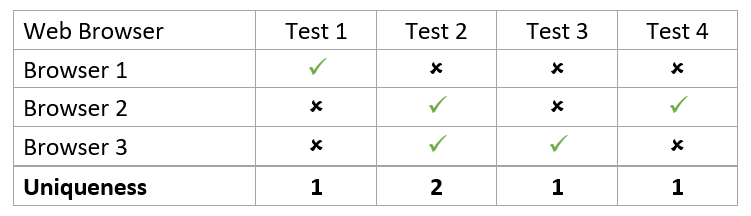
\includegraphics[width=300pt, height=80pt]{MinimalFP.png}
	\caption{Example for the structure of a minimal fingerprint\\}
	\label{MinimalFP}
\end{figure}
If the test set is rather large it is more effective to use a \textit{binary decision tree}. This method runs multiple test rounds to determine a web browser and major version. There is no need for a unique fingerprint as the tests split the browsers to identify them. Therefore there is no need to run a test for each browser and version unlike the minimal fingerprint which reduces the total number of executed tests. (\textcite{mulazzani13}, p.4)\\\\
\autoref{DecisionTree} gives a good overview of how such a tree can be structured. The leaf nodes pose as browsers, the inner nodes display the used tests and the edges indicate the success. (\textcite{mulazzani13}, p.4)
\begin{figure}[H]
	\centering
	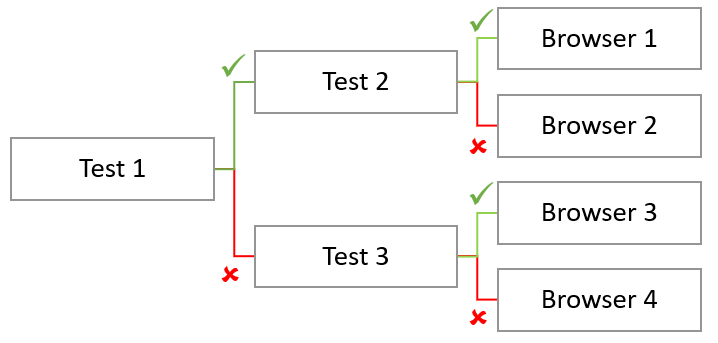
\includegraphics[width=290pt, height=120pt]{DecisionTree.png}
	\caption{Example for the structure of a decision tree}
	\label{DecisionTree}
\end{figure}
%weaknesses?
\begin{comment}
--  having a comparable overhead for creating and collecting fingerprint samples.
-- implemented in just a few hundred lines of JS
-- undetectable for the user - CPU not stalled noticeably
(\textcite{mulazzani13}, p.2)
-- used to detect modified User-Agent strings, and can be used to reliably identify the browser of Tor Browser Bundle users.
(\textcite{upi15}, p.2)
\end{comment}
\subsection{Cross-Browser fingerprinting}
In 2011 Boda et al. conducted the first study on cross-browser fingerprinting, utilizing a part of the user's IP address as part of the fingerprint. Even though this technique is not optimal, as the IP address can be modified by e.g. proxies, it remained the only paper published this kind of fingerprinting until Cao et al. published an improved version in 2017. (\textcite{boda11}, p.14)(\textcite{Cao17}, p.1)

\subsubsection{How it works}
Cross-Browser fingerprinting uses browser-independent features to track a user regardless of the browser they are using. This can be done by relying only on the use of JavaScript and font detection. (\textcite{upi15}, pp.2)\\\\
%The fingerprint is created from specific browser data with the help of JavaScript and server-side algorithms.(\textcite{boda11}, p.4)
To be able to track a user across different web browsers a set of browser-independent features is used as a basis of identification. Part of this set is for example (\textcite{boda11}, p.2)
\begin{itemize}
	\item networking information (ip address, hostname, TCP port number)
	\item application layer information (user agent string, name and version of the operating system, extensions)
	\item information gained by quering (list of fonts, screen resolution, timezone, plug-ins and their version)\\
\end{itemize}
The difference to other fingerprints is that the first two octets of the IP address are used, which usually remain constant even if the IP address of the client changes dynamically. The downside is that it may change when switching ISP or other services. (\textcite{boda11}, p.5)\\\\
%uses locality, short user id(script-generated identifier, derived from the first two octets of the IP address), usa, os, screen, timezone, basic fonts, all fonts, browser name and version (\textcite{boda11}, p.5)
Besides, the IP address is modified by proxies for privacy reasons, which changes the unique fingerprint. Boda et al. dealt with that problem saying that the other parameters suffice to identify a user.\\\\
Cao et al. improved this method by excluding the IP address, modifying the use of some data and adding some features.(\textcite{Cao17}, p.1) This technique forces the system to perform 36 tasks which return the required information in less than a minute.\\\\
This fingerprinting technique is based on different novel operating systems and hardware level features (e.g. from graphic card, CPU, audio stack, and installed writing scripts). Many of these features are exposed to JavaScript over web browser APIs, which are used to extracted them.(\textcite{Cao17}, pp.1)\\\\
\begin{comment}
99,24\%  successfully identify users 
83.24\% uniqueness with 91.44\% cross-browser stability(\textcite{Cao17}, p.2)
compared to Boda excluding ip address -68.98\% uniqueness with 84.64\% cross-browser stability.
\end{comment}
Some improvements Cao et al. made towards Boda et al.'s technique are:
\begin{tcolorbox}
	Improvement 1:\\
	Change of the screen resolution. In browsers like Firefox and Internet Explorer the resolution changes when the user zooms. Therefore this method takes the zoom level into consideration and normalizes the width and height of the screen resolution. (\textcite{Cao17}, p.2)
\end{tcolorbox}
\begin{tcolorbox}
	Improvement 2:\\
	The formats DataUrl and JPEG are unstable across different browsers, therefore Cao et al. prefered the use of a lossless format like PNG. (\textcite{Cao17}, p.2)
\end{tcolorbox}
The script sends various rendering tasks (e.g. drawing curves and lines to client side) and also obtains operating system and hardware level information. The client side browser renders and returns the results (images, sound waves) which are converted into hashes. In the meantime the browser collects browser-specific information.(\textcite{Cao17}, p.4)\\\\
The final fingerprint is generated from a list of hashes which is intertwined with a mash with the help of an "and"-operation. The mask consists of collected browser information, whereas each browser has its own mask. (\textcite{Cao17}, p.4)\\\\
Contrary to single browser techniques cross-browser fingerprinting has no problem identifying users across browsers. Anyway, it has the same weakness as all fingerprints: identically configured devices. (\textcite{upi15}, pp.2)

\begin{comment}
-- nr of CPU virtual cores - obtained by browser feature "hardwareConcurrency"
-- audiocontext - provides bundle of audio signal processing functionalities from signal generation to signal
--peak values and their corresponding frequencies are relatively stable
across browsers. 
-- create a list of bins with small steps on both the frequency and value axes, and map the peak
frequencies and values to the corresponding bins.
-- If one bin contains a frequency or value, we mark the bin as one and
otherwise zero: such list of bins serve as our cross-browser feature.
-- List of Fonts width and height of a certain string is measured to determine font type
-- Line, curve, and anti-aliasing. Line and curve are 2D features
supported by both Canvas (2D part) and WebGL.
--Vertex shader. A vertex shader, rendered by GPU and the
driver, converts each vertex in a 3D model to its coordinate in
a 2D clip-space.
-- Fragment shader. A fragment shader, rendered by GPU and
the driver as well, processes a fragment, such as a triangle
outputted by the rasterization, into a set of colors and a single
depth value.
--- MANY MORE - not write down all, als need to cut short - max. 1page per technique!!!!

%4 features for cross-browser fp (screen res., color depth, list of fonts, platform)
(\textcite{Cao17}, p.3)
\end{comment}